\thispagestyle{empty}
%
% This is the cover artwork, made with Tikz graphic language
%
\begin{tikzpicture}[remember picture,overlay]
  %% Catch some significant points on the borders of the page
  \coordinate (p1) at (current page.south west); % lower left corner
  \coordinate (p2) at ($(p1)+(\paperwidth,0)$); % lower right
  \coordinate (p3) at ($(p2)+(0,\paperheight)$); % upper right
  \coordinate (p4) at ($(p1)+(0,\paperheight)$); % upper left
  \coordinate (m1) at ($(p1)!0.5!(p2)$); % midway of lower side
  \coordinate (m2) at ($(p2)!0.5!(p3)$); % midway of right side
  \coordinate (m3) at ($(p3)!0.5!(p4)$); % midway of upper side
  \coordinate (m4) at ($(p4)!0.5!(p1)$); % midway of left side

  %% Paint the two halves of the sheet in red and black
  \fill[Aquamarine!30] (m4) rectangle (p3);
  \fill[NavyBlue!100] (p1) rectangle (m2);
  
  %% Cover image
  \node[
    % http://tex.stackexchange.com/questions/11272/faded-drop-shadow-using-tikz-based-rounded-rectangle
    % TO DO: drop a shadow with pgf-blur
    %
    anchor=south east, opacity=1.0, NavyBlue, xshift=-10mm, yshift=55mm] at (m2) {%
    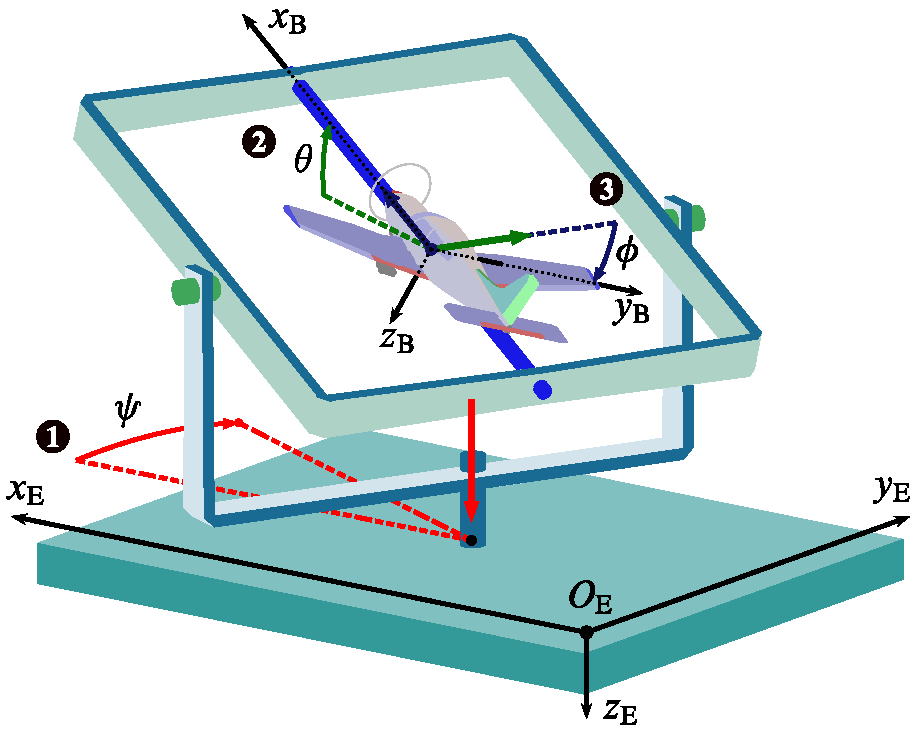
\includegraphics[%
      trim = 0mm 0mm 0mm 0mm,% left  bottom  right  top
      clip,% actually cut what trim says
      width=0.50\paperwidth]{cover_ac_euler_gimbal.pdf}%
  };
  
  %% Anchor to the point midway on the right side of the page
  %% and position all the elements accordingly
  \node[
    % http://tex.stackexchange.com/questions/11272/faded-drop-shadow-using-tikz-based-rounded-rectangle
    % TO DO: drop a shadow with pgf-blur
    %
    anchor=south east, opacity=1.0, NavyBlue!100!black, xshift=-1.0cm, yshift=0.6cm] at (m2) {%
    %\fontsize{46}{48}\selectfont% allowed by Type 1 fonts
    \fontsize{38}{40}\selectfont%
    \bfseries 
    \parbox{1.00\paperwidth}{\raggedleft \myDocName}
  };
  \node[anchor=north east, opacity=1.0, white, xshift=-1.0cm, yshift=-0.8cm] at (m2) {%
    \fontsize{32}{34}\selectfont%
    \bfseries
    \parbox{1.00\paperwidth}{\raggedleft \myDocSubTitle}
  };
%   \node[anchor=north east, opacity=1.0, Aquamarine!40!white, xshift=-1.0cm, yshift=-5.5cm] at (m2) {%
%     \parbox{0.5\linewidth}{%
%     \raggedleft\fontsize{46}{48}\selectfont\bfseries%
%     DSV}};
  \node[anchor=north east, opacity=1.0, white, xshift=-1.0cm, yshift=-9.0cm] at (m2) {%
    \parbox{0.5\linewidth}{%
    \Huge\raggedleft
    Andrea Grande}};
  \node[anchor=north west, opacity=1.0, white, xshift=1.0cm, yshift=-12.5cm] at (m4) {%
    \parbox{0.5\linewidth}{%
      %\Huge
      %\myDocDate\\[0.5em]
      \begin{tcolorbox}[hbox, colback=magenta, colframe=magenta]
        \color{white}\texttt{\myDocVersion} --- \myDocDate
      \end{tcolorbox}
    }};    
\end{tikzpicture}